\chapter{Anhang}
\label{ch:anhang}

\section{Lösungsansatz}
\label{sec:anhang-loesungsansatz}

\begin{figure}[htb]
	\centering
	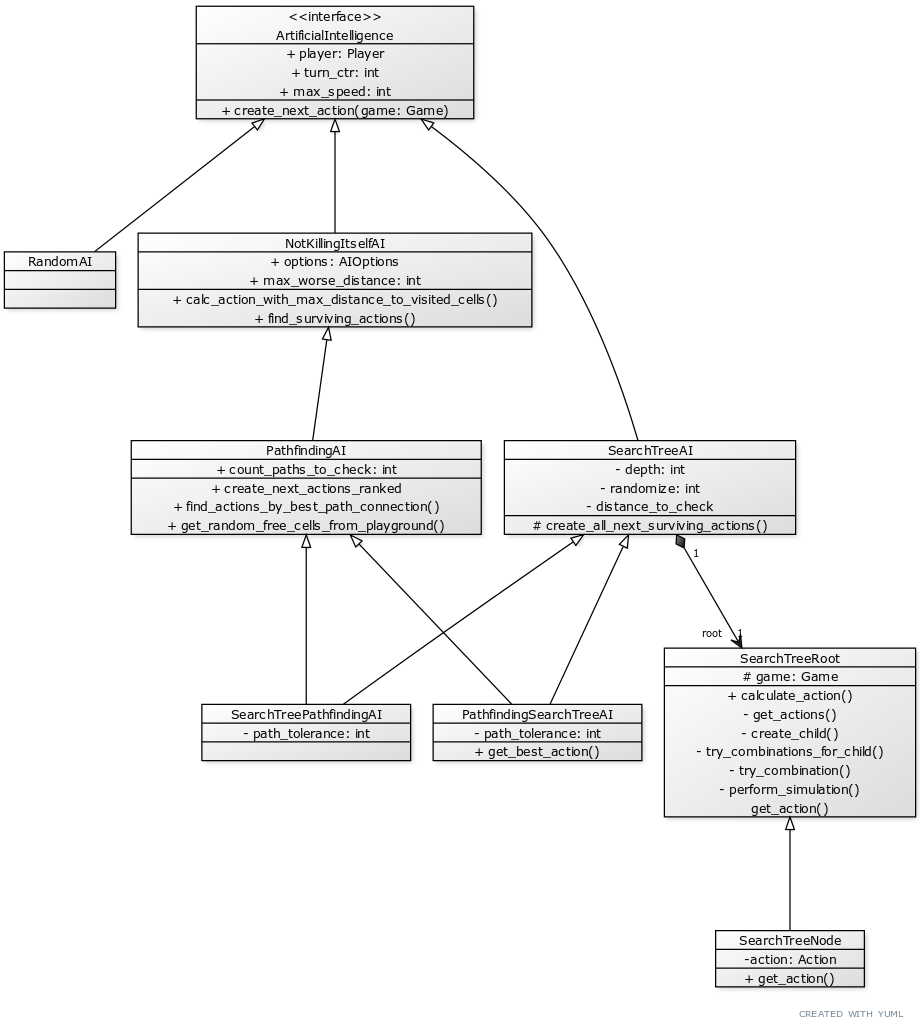
\includegraphics[width=0.8\textwidth]{Bilder/Klassendiagramm_AIs.png}
	\caption{UML-Klassendiagramm der \ac{KI}s}
	\label{fig:klassendiagramm-AIs}
\end{figure}
\clearpage

\section{Implementierung}
\label{sec:anhang-implementierung}

\begin{figure}[htb]
	\centering
	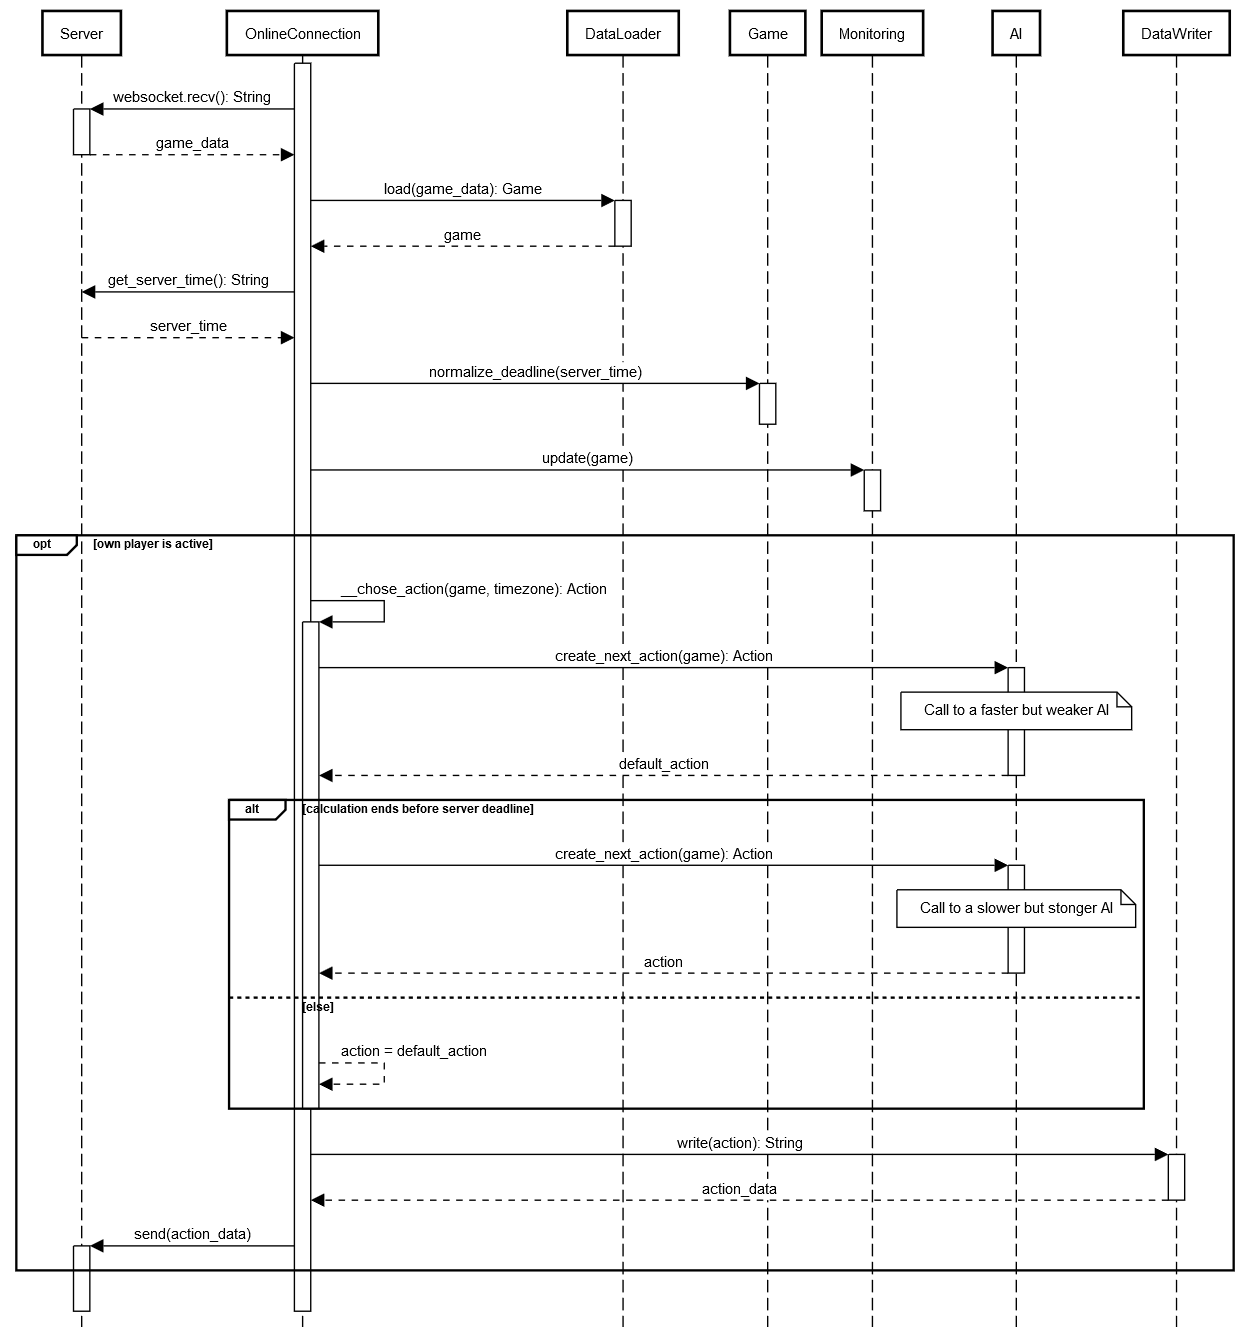
\includegraphics[width=\textwidth]{Bilder/Sequenzdiagramm_Implementierung_Spielzug.png}
	\caption{Sequenzdiagramm zur Implementierung eines Spielzug}
	\label{fig:sequenzdiagramm-spielzug}
\end{figure}
\clearpage

\begin{minipage}{\textwidth}
	\lstinputlisting[label=lst:online-__play,style=pythonstyle,caption=\Code{\_\_play()}-Methode des \Code{OnlineController}s]
	{./Dokumente/OnlineController-__play.txt}
\end{minipage}
\clearpage

\begin{minipage}{\textwidth}
	\lstinputlisting[label=lst:json-spiel,caption=JSON-Repräsentation eines Spiel-Zustands]
	{./Dokumente/game_beispiel.json}
\end{minipage}
\clearpage

\begin{figure}[htb]
	\centering
	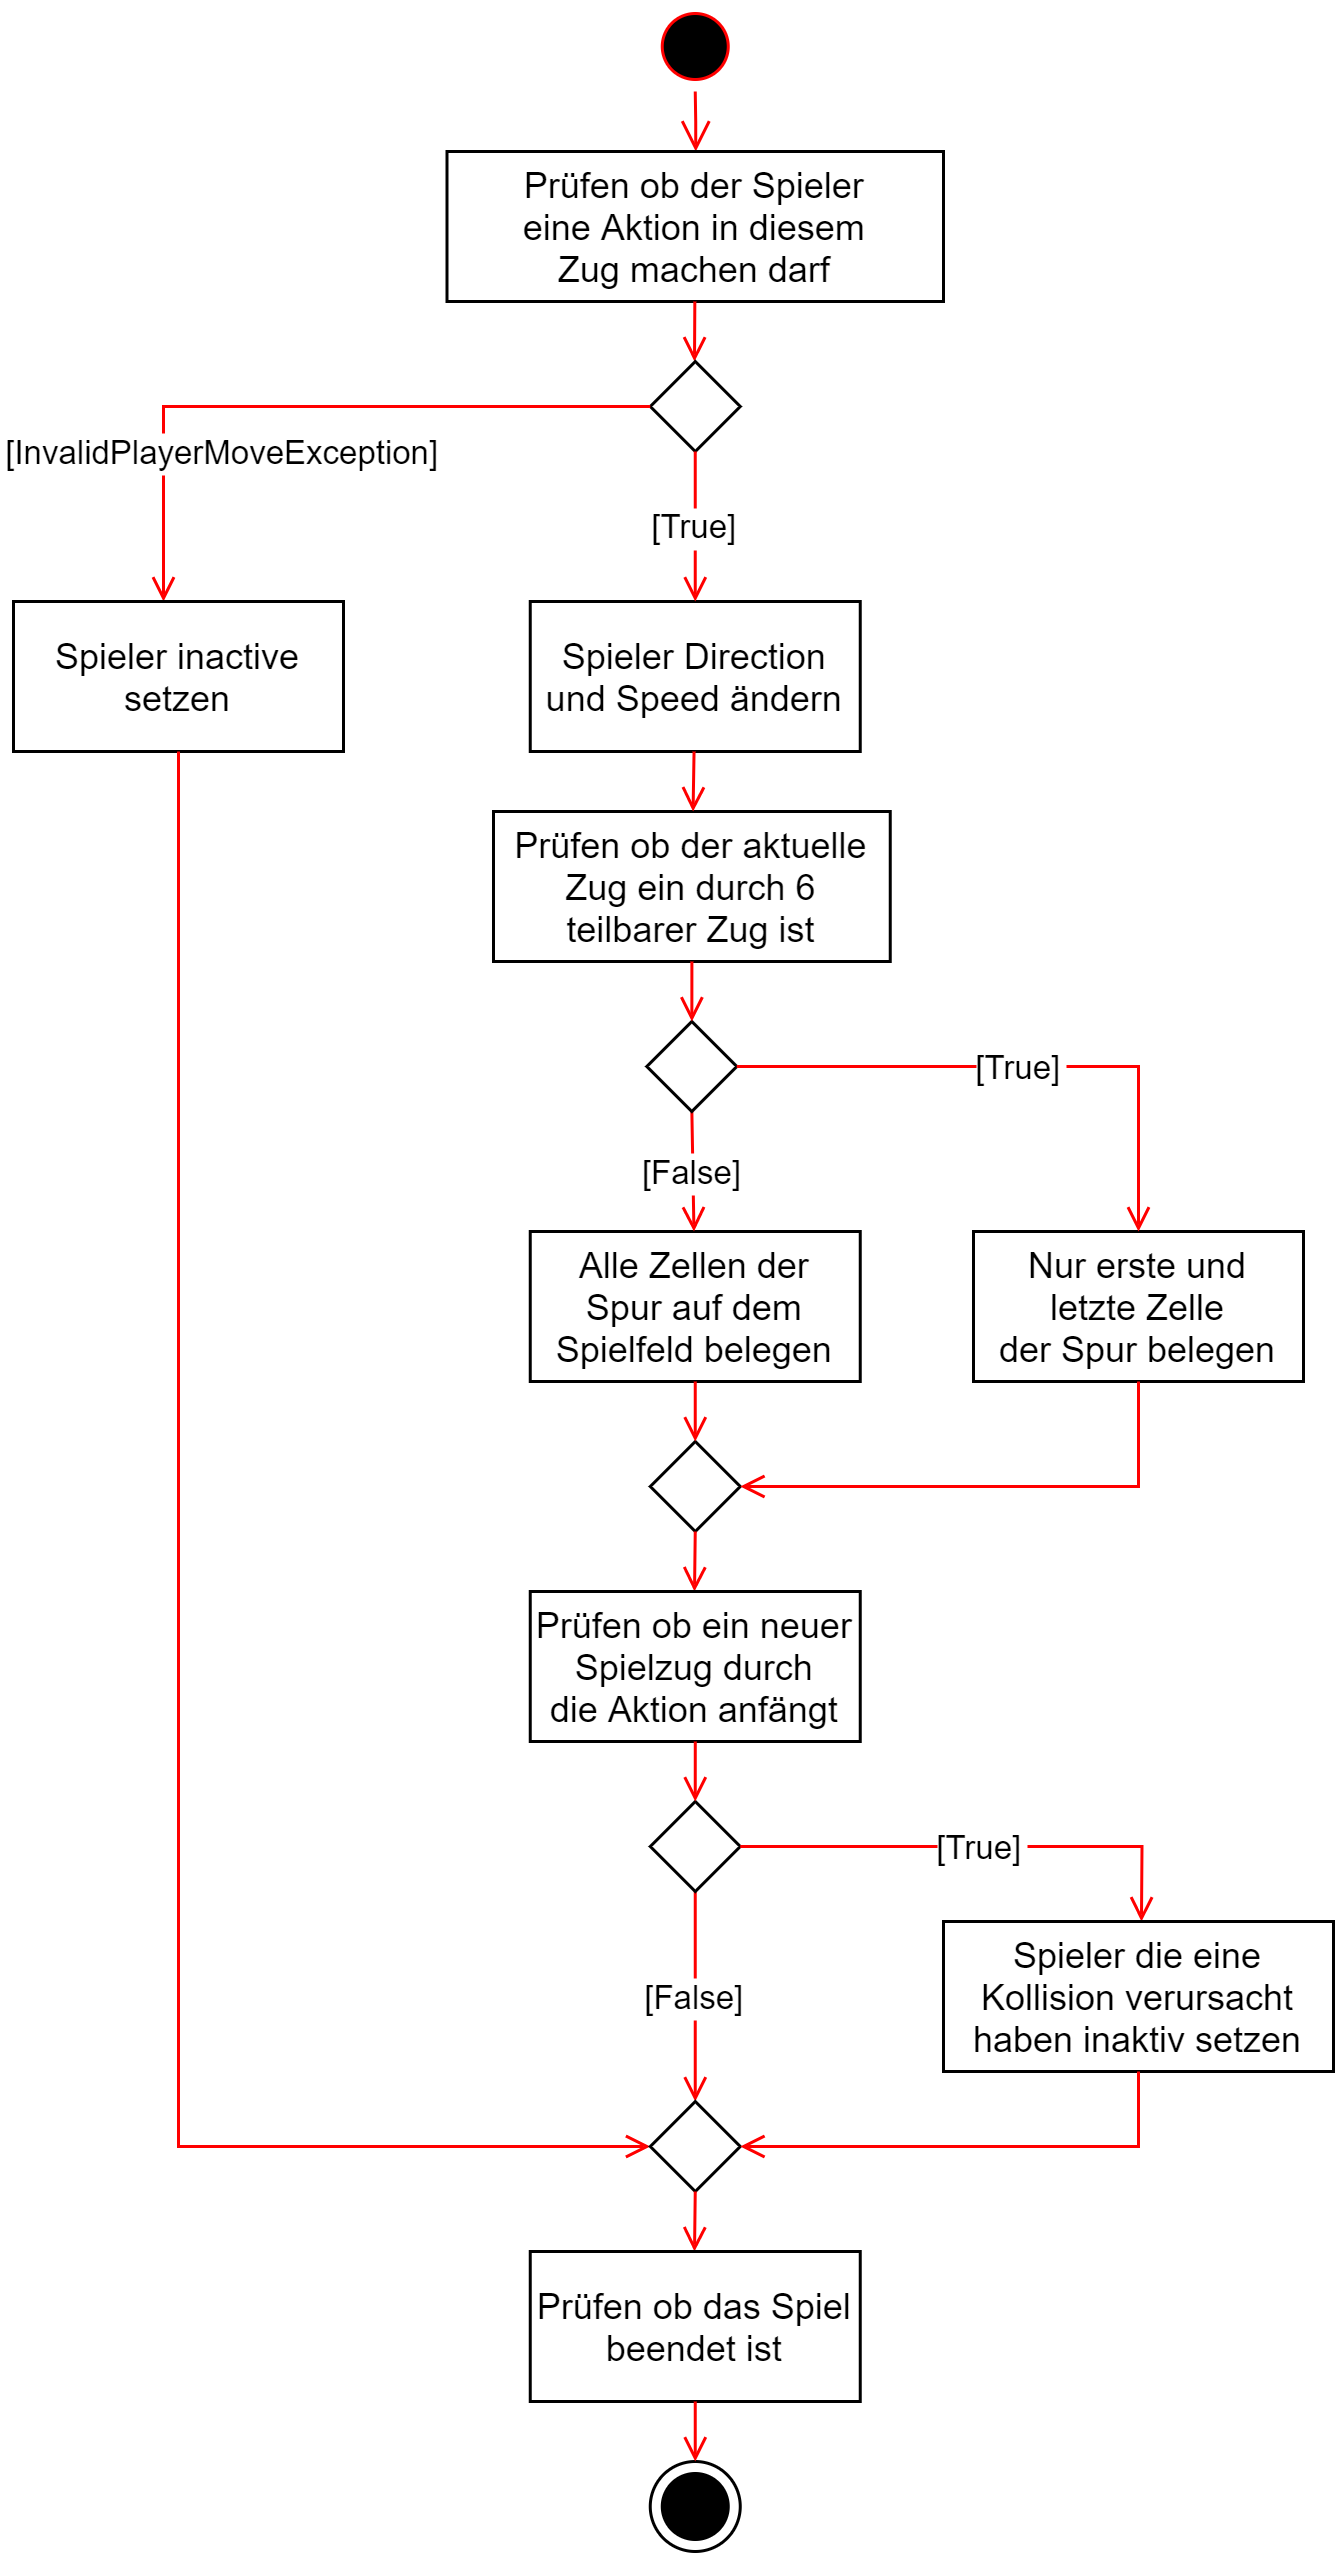
\includegraphics[width=0.7\textwidth]{Bilder/game_service_do_action_activity_diagram.png}
	\caption{Aktivitätsdiagramm zur Durchführung einer Spieler-Aktion durch den \Code{GameService}}
	\label{fig:aktivitaetsdiagramm-spieleraktion-gameservice}
\end{figure}
\clearpage

\begin{minipage}{\textwidth}
	\lstinputlisting[label=lst:get-and-visit-cells
	,style=pythonstyle,caption=\Code{get\_and\_visit\_cells(player, action)}-Methode des \Code{GameService}]
	{./Dokumente/Get_And_Visit_Cells_GameService.txt}
\end{minipage}
\clearpage

\begin{minipage}{\textwidth}
	\lstinputlisting[label=lst:pygame_update
	,style=pythonstyle,caption=\Code{update(game: Game)}-Methode der \Code{GraphicalView}]
	{./Dokumente/graphicalview_update.txt}
\end{minipage}
\clearpage

\section{Evaluation}
\label{sec:anhang-evaluation}

\lstinputlisting[label=lst:eval-sql-1,style=sqlstyle,caption=Auswertung der besten \ac{KI}-Klasse]
{./Dokumente/ai_evaluation_1.sql}
\clearpage

\lstinputlisting[label=lst:eval-sql-2,style=sqlstyle,caption=Auswertung der besten \ac{KI}-Konfiguration]
{./Dokumente/ai_evaluation_2.sql}
\clearpage

\section{Weiterentwicklung}
\label{sec:anhang-weiterentwicklung}

\begin{minipage}{\textwidth}
	\lstinputlisting[label=lst:yaml-github-action,style=githubactionstyle,caption=YAML-Konfiguration der Github Action]
	{../.github/workflows/python-app.yml}
\end{minipage}
\clearpage
